 \documentclass[sigconf]{acmart}

 % Used to create latex table
%  https://www.tablesgenerator.com/latex_tables#

 %% ----------------------------------------------------------------
%% Packages
%% ----------------------------------------------------------------
\usepackage{balance}

%% ----------------------------------------------------------------
%% Commands
%% ----------------------------------------------------------------
\newcommand{\cmt}[2][red]{ {\color{#1} XXX: #2} }
% \renewcommand{\figurename}{Fig.}
% \renewcommand{\sectionname}{Section}

%% ----------------------------------------------------------------
%% Conference info and paper info
%% ----------------------------------------------------------------
\setcopyright{acmcopyright}
\copyrightyear{2018}
\acmYear{2018}
\acmDOI{10.1145/1122445.1122456}

\acmConference[Woodstock '18]{Woodstock '18: ACM Symposium on Neural
  Gaze Detection}{June 03--05, 2018}{Woodstock, NY}
\acmBooktitle{Woodstock '18: ACM Symposium on Neural Gaze Detection,
  June 03--05, 2018, Woodstock, NY}
\acmPrice{15.00}
\acmISBN{978-1-4503-XXXX-X/18/06}


%% ----------------------------------------------------------------
%% Document content
%% ----------------------------------------------------------------
\begin{document}
\title{XXX}

% For the  double-blind review
\author{Anonymous authors}
\orcid{xxxx-xxxx-xxxx-xxxx}
 \affiliation{
    \institution{Paper under double-blind review}
    \streetaddress{}
    \city{}
    \state{}
    \country{}
    \postcode{}
 }
 \email{}
\renewcommand{\shortauthors}{Anonymous Author, et al.}

\begin{abstract}

Abstract content.

\end{abstract}

% The code below should be generated by the tool at
% http://dl.acm.org/ccs.cfm
% Please copy and paste the code instead of the example below. 
\begin{CCSXML}
<ccs2012>
    <concept>
        <concept_id>10010520.10010521.10010542.10010294</concept_id>
        <concept_desc>Computer systems organization~Neural networks</concept_desc>
        <concept_significance>300</concept_significance>
    </concept>
    <concept>
        <concept_id>10011007.10011006.10011041.10011047</concept_id>
        <concept_desc>Software and its engineering~Source code generation</concept_desc>
        <concept_significance>500</concept_significance>
    </concept>
    <concept>
        <concept_id>10002978.10003022</concept_id>
        <concept_desc>Security and privacy~Software and application security</concept_desc>
        <concept_significance>500</concept_significance>
    </concept>
</ccs2012>
\end{CCSXML}
    
\ccsdesc[300]{Computer systems organization~Neural networks}
\ccsdesc[500]{Software and its engineering~Source code generation}
\ccsdesc[500]{Security and privacy~Software and application security}

%% ----------------------------------------------------------------
%% Keywords
%% ----------------------------------------------------------------
\keywords{Privacy-preserving inference; deep neural networks; deep neural network compilation; secure two-party computation}

\maketitle

%% ----------------------------------------------------------------
%% Introduction
%% ----------------------------------------------------------------
\section{Introduction} \label{introduction}

Test \cite{XXX}.

%% ------------------------------------------------------------
%% Background
%% ------------------------------------------------------------
\section{Background} \label{background}

\subsection{XXX}

%% ------------------------------------------------------------
%% Methodology
%% ------------------------------------------------------------
\section{Methodology}

\begin{figure}[b]
    \centering
    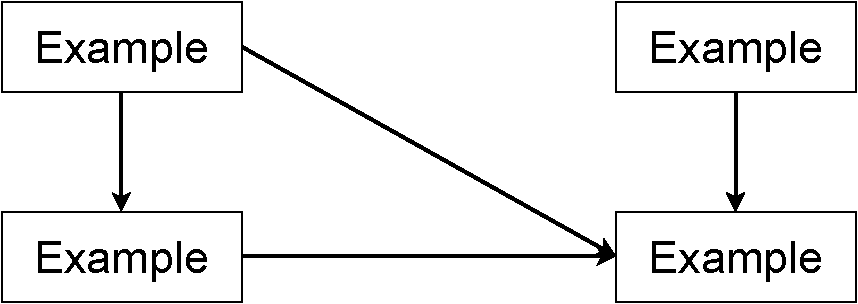
\includegraphics[width=.75\linewidth]{figures/paper-example.pdf}
    \caption{Test.}
    \Description{}
    \label{fig:overview}
\end{figure}

%% ------------------------------------------------------------
%% Evaluation
%% ------------------------------------------------------------
\section{Experimental Results} \label{evaluation}

%% ------------------------------------------------------------
%% Related Work
%% ------------------------------------------------------------
\section{Related Work} \label{related_work}


%% ------------------------------------------------------------
%% Conclusions
%% ------------------------------------------------------------
\section{Conclusion} \label{conclusion}


%% ----------------------------------------------------------
%% Acknowledgments
%% ----------------------------------------------------------
% \begin{acks}

% \end{acks}
\balance
\bibliographystyle{ACM-Reference-Format}
\bibliography{paper} 

\end{document}